\documentclass[11pt]{article}
\usepackage{fullpage}
\usepackage{hyperref}


\usepackage[english]{babel}
\usepackage[latin1]{inputenc}

\usepackage{times}
\usepackage[T1]{fontenc}

\usepackage{color}
\usepackage{colortbl}
%\usepackage{graphicx}
\usepackage{alltt}
\usepackage{marvosym}
\usepackage{pgf}
\usepackage{tikz}
%\usetikzlibrary{arrows,snakes,backgrounds}

\tikzstyle{element}=[rectangle,draw=black,fill=black!20,minimum size=1cm]
\tikzstyle{emptyel}=[rectangle,draw=black,fill=white,minimum size=1cm]
\tikzstyle{ghostel}=[rectangle,draw=white!20,fill=white!20,minimum size=1cm]
\tikzstyle{vertex}=[circle,draw=blue!50,fill=blue!20,minimum size=1cm]

%\setbeamercolor{highback}{bg=yellow}
%\setbeamercolor{nighnone}{}

\newcommand{\high}[1]{\alert<.>{#1}}
\newcommand{\highin}[2]{\alert<#1>{#2}}
\newcommand{\ithi}[1]{\item \alert<.>{#1}}
\newcommand{\rahi}[1]{\item[$\rightarrow$] \alert<.>{#1}}
\newcommand{\Rahi}[1]{\item[$\Rightarrow$] \alert<.>{#1}}
\newcommand{\qa}[5]{\only<#1>{#2}\only<#3>{#4}}
\newcommand{\tinyh}[1]{#1}

% Style definition file generated by highlight 2.13, http://www.andre-simon.de/ 

% Highlighting theme definition: 

\newcommand{\hlstd}[1]{\textcolor[rgb]{0,0,0}{#1}}
\newcommand{\hlnum}[1]{\textcolor[rgb]{0.16,0.16,1}{#1}}
\newcommand{\hlesc}[1]{\textcolor[rgb]{1,0,1}{#1}}
\newcommand{\hlstr}[1]{\textcolor[rgb]{1,0,0}{#1}}
\newcommand{\hldstr}[1]{\textcolor[rgb]{0.51,0.51,0}{#1}}
\newcommand{\hlslc}[1]{\textcolor[rgb]{0.51,0.51,0.51}{\it{#1}}}
\newcommand{\hlcom}[1]{\textcolor[rgb]{0.51,0.51,0.51}{\it{#1}}}
\newcommand{\hldir}[1]{\textcolor[rgb]{0,0.51,0}{#1}}
\newcommand{\hlsym}[1]{\textcolor[rgb]{0,0,0}{#1}}
\newcommand{\hlline}[1]{\textcolor[rgb]{0.33,0.33,0.33}{#1}}
\newcommand{\hlkwa}[1]{\textcolor[rgb]{0,0,0}{\bf{#1}}}
\newcommand{\hlkwb}[1]{\textcolor[rgb]{0.51,0,0}{#1}}
\newcommand{\hlkwc}[1]{\textcolor[rgb]{0,0,0}{\bf{#1}}}
\newcommand{\hlkwd}[1]{\textcolor[rgb]{0,0,0.51}{#1}}
\definecolor{bgcolor}{rgb}{1,1,1}



%% Uncomment this, if you want the table of contents to pop up at
%% the beginning of each subsection:
%\AtBeginSubsection[]
%{
%  \begin{frame}<beamer>{Outline}
%    \tableofcontents[currentsection,currentsubsection]
%  \end{frame}
%}

% If you wish to uncover everything in a step-wise fashion, uncomment
% the following command: 

%\beamerdefaultoverlayspecification{<+->}

% If you have a file called "university-logo-filename.xxx", where xxx
% is a graphic format that can be processed by latex or pdflatex,
% resp., then you can add a logo as follows:

% \pgfdeclareimage[height=0.5cm]{university-logo}{university-logo-filename}
% \logo{\pgfuseimage{university-logo}}


\newcommand{\anders}{Anders Jonsson}
\newcommand{\email}{\texttt{anders.jonsson@upf.edu}}

\newcommand{\ddate}{2010-2011}
\newcommand{\Cpp}{{\tt C++}}

\newcommand{\compcpp}[3]{\item{\high{#1} \begin{itemize} \item[ObjC] #2 \item[C++] #3\end{itemize}}}
\newcommand{\hashinc}[1]{\#include\textless #1\textgreater}
%\newcommand{\jfinc}[1]{{\tiny\verbatiminput{src/#1}}}   % this can be switched to \tiny\input .tex if highlight works
\newcommand{\jfinc}[1]{{\tiny\input{#1}}}

\usepackage{amssymb}
\usepackage{mathtools}
\usepackage{amsthm}
\usepackage{multirow}
\usepackage{pgfplots}
\usepackage{tikz}
\usetikzlibrary{arrows,automata,positioning}
\usetikzlibrary{shapes.multipart}
\usetikzlibrary{decorations.markings}
\usetikzlibrary{decorations.pathreplacing}
\usetikzlibrary{intersections, pgfplots.fillbetween}

\setlength{\textheight}{11.00in}
\setlength{\topmargin}{-0.2in}

\title{
\vspace{-1.2cm}
Machine Learning 2020-21\\ Final Exam}
\author{15 December 2020}
\date{Name: \dotfill}% NIA: \dotfill}

\newcounter{marks}
\setcounter{marks}{0}

\def\ci{\perp\!\!\!\perp}

\begin{document}

\maketitle

\newcounter{PreguntaCounter}

\begin{list}{{\bf Question \arabic{PreguntaCounter}:}}
	{\usecounter{PreguntaCounter}
	}

\item
\fbox{2 points}
\addtocounter{marks}{2}
In linear regression with L2 regularization, the augmented training loss is \[L_{\mathrm{aug}}(w)=\frac 1 m (w^\top\mathrm{X}^\top\mathrm{X}w - 2w^\top\mathrm{X}^\top y + y^\top y + \lambda w^\top w),\] and the optimal weight vector is $w_{\mathrm{reg}}=(\mathrm{X}^\top\mathrm{X} + \lambda I)^{-1}\mathrm{X}^\top y$. What is the augmented training loss of $w_{\mathrm{reg}}$? Show the entire derivation and simplify the expression as much as possible.

\framebox[16cm][l]{ 
\parbox{15.9cm}{
\vspace*{7cm}
}}

\item
\fbox{2 points}
\addtocounter{marks}{2}
A company develops an application that estimates how long it will take users to drive to work. To do so, the company collects data of users driving to work, recording the initial and final location of the drive, and the time of day at the beginning and at the end. Which type of machine learning problem is this, and how are the concrete components of this learning problem defined?

\framebox[16cm][l]{ 
\parbox{15.9cm}{
\vspace*{6.5cm}
}}

\pagebreak

\begin{center}
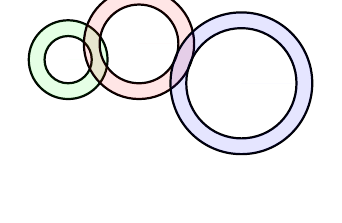
\begin{tikzpicture}
 	\draw[name path=E,thick] (0.3,0.8) circle (0.3cm);
 	\draw[name path=F,thick] (0.3,0.8) circle (0.5cm);
	\tikzfillbetween[of=E and F]{green, opacity=0.1};
 	\draw[name path=A,thick] (1.2,1) circle (0.5cm);
 	\draw[name path=B,thick] (1.2,1) circle (0.7cm);
	\tikzfillbetween[of=A and B]{red, opacity=0.1};
 	\draw[name path=C,thick] (2.5,0.5) circle (0.7cm);
 	\draw[name path=D,thick] (2.5,0.5) circle (0.9cm);
	\tikzfillbetween[of=C and D]{blue, opacity=0.1};
\end{tikzpicture}
\end{center}

\item
\fbox{1 point}
\addtocounter{marks}{1}
Consider an input space in two dimensions in which the true concept classes are defined as (possibly overlapping) circular bands, as shown in the figure. Now imagine that you sample many data points from this input space, such that each data point falls within one of the circular bands. However, you do not have access to labels. If you wanted to perform unsupervised learning for this problem, which concrete algorithm would you choose, and why?

\framebox[16cm][l]{ 
\parbox{15.9cm}{
\vspace*{5cm}
}}

\item
\fbox{1 point}
\addtocounter{marks}{1}
How is the bias-variance tradeoff defined? Give an example of a learning problem with low bias, and a learning problem with low variance, and use the examples to discuss the tradeoff.

\framebox[16cm][l]{ 
\parbox{15.9cm}{
\vspace*{5cm}
}}

\item
\fbox{1 point}
\addtocounter{marks}{1}
What is the meaning of the ``kernel trick''? Describe how the kernel trick is applied in machine learning, and why it is important.

\framebox[16cm][l]{ 
\parbox{15.9cm}{
\vspace*{5cm}
}}



\pagebreak

Name: \dotfill

\item
\fbox{2 point}
\addtocounter{marks}{1}
Given some dataset $\mathcal{D}$ and some model hypothesis parameterized by parameters~$\theta$, explain three main differences between estimating $\theta$ using Bayesian estimation and maximum likelihood. Illustrate the Bayesian approach with an example.

\framebox[16cm][l]{ 
\parbox{15.9cm}{
\vspace*{9cm}
}}

\item
\fbox{2 point}
\addtocounter{marks}{1}
We want to learn a generative model of text from a large corpus comprising senteces of different length in natural language.
As a first approximation, we assume that the probability of a letter $X_k$ depends essentially on the two letters that appeared previously in the text, $X_{k-1}$ and $X_{k-2}$. Describe a Bayesian network representing such a model and then transform it into a factor graph.
Formalize two conditional independencies that are derived from such a model.

\framebox[16cm][l]{ 
\parbox{15.9cm}{
\vspace*{9cm}
}}



\pagebreak

Name: \dotfill

\item
\fbox{1 point}
\addtocounter{marks}{1}
In discounted Markov decision processes, the value function $V^\pi$ associated with a deterministic policy $\pi:\mathcal{X}\rightarrow \mathcal{A}$ is defined as $V^\pi(x) = \mathbb{E}_\pi\left[\sum_{t=0}^\infty \gamma^t r_t\middle| x_0 = x\right]$
for all states $x\in\mathcal{X}$. Using this notation, give the definition of an optimal policy $\pi^*$ and the optimal value function $V^*$.

\framebox[16cm][l]{ 
\parbox{15.9cm}{
\vspace*{4.5cm}
}}

\item
\fbox{1 point}
\addtocounter{marks}{1}
The Value Iteration algorithm for discounted Markov decision processes iteratively computes a sequence of value functions $V_1,V_2,\dots,V_k$. In a given iteration $k$ of the algorithm, what is the relation between $V_{k}$ and $V_{k+1}$?

\framebox[16cm][l]{ 
\parbox{15.9cm}{
\vspace*{5cm}
}}

\item
\fbox{2 points}
\addtocounter{marks}{2}
Describe the TD(0) algorithm for policy evaluation in discounted Markov decision processes. If the algorithm is luckily initialized with the true value function $\widehat{V}_0 = V^\pi$, what is the expectation of $\widehat{V}_1$?

\framebox[16cm][l]{ 
\parbox{15.9cm}{
\vspace*{7.5cm}
}}


\end{list}


\end{document}
